\documentclass[conference]{IEEEtran}

\ifCLASSINFOpdf
  \usepackage[pdftex]{graphicx}
\else
  \usepackage[dvips]{graphicx}
\fi
\usepackage{amsmath}
\usepackage{amssymb}
\usepackage{balance}
\usepackage[usenames,dvipsnames,svgnames,table]{xcolor}
\usepackage{algpseudocode}
% \usepackage{minipages}

\newcommand{\compactimg}{\vspace{-10pt}}
\newcommand{\tableref}[1]{Table~\ref{tab:#1}}
\newcommand{\figref}[1]{Figure~\ref{fig:#1}}
\newcommand{\secref}[1]{Section~\ref{sec:#1}}
\newcommand{\algoref}[1]{Algorithm~\ref{algo:#1}}

\hyphenation{}

\begin{document}

\title{Demo Abstract: The OpenChirp Low-Power Wide-Area Network and Ecosystem}
\author{
	\IEEEauthorblockN{Adwait Dongare, Anh Luong, Artur Balanuta, Craig Hesling, Khushboo Bhatia, Anthony Rowe}
	\IEEEauthorblockA{
		Electrical and Computer Engineering Department\\
		Carnegie Mellon University, Pittsburgh PA\\
	}
}

% conference papers do not typically use \thanks and this command
% is locked out in conference mode. If really needed, such as for
% the acknowledgment of grants, issue a \IEEEoverridecommandlockouts
% after \documentclass

% for over three affiliations, or if they all won't fit within the width
% of the page, use this alternative format:
% 
%\author{\IEEEauthorblockN{Michael Shell\IEEEauthorrefmark{1},
%Homer Simpson\IEEEauthorrefmark{2},
%James Kirk\IEEEauthorrefmark{3}, 
%Montgomery Scott\IEEEauthorrefmark{3} and
%Eldon Tyrell\IEEEauthorrefmark{4}}
%\IEEEauthorblockA{\IEEEauthorrefmark{1}School of Electrical and Computer Engineering\\
%Georgia Institute of Technology,
%Atlanta, Georgia 30332--0250\\ Email: see http://www.michaelshell.org/contact.html}
%\IEEEauthorblockA{\IEEEauthorrefmark{2}Twentieth Century Fox, Springfield, USA\\
%Email: homer@thesimpsons.com}
%\IEEEauthorblockA{\IEEEauthorrefmark{3}Starfleet Academy, San Francisco, California 96678-2391\\
%Telephone: (800) 555--1212, Fax: (888) 555--1212}
%\IEEEauthorblockA{\IEEEauthorrefmark{4}Tyrell Inc., 123 Replicant Street, Los Angeles, California 90210--4321}}




% use for special paper notices
%\IEEEspecialpapernotice{(Invited Paper)}




% make the title area
\maketitle

\begin{abstract}

In this demonstartion, we first present OpenChirp, an open-source Low-Power
Wide Area Networking (LPWAN) infrastructure. OpenChirp provides a
completely open-source framework for a simple and rapidly deployable
internet-of-things (IoT) network that is also stable, modular and scaleable.
With a focus to enable research on the wireless physical layer, we also
present LPRAN, a low-cost high-performance software-defined radio hardware
platform that can receive signals up to -30~dB below the noise floor.

\end{abstract}

\IEEEpeerreviewmaketitle

% \section{Introduction}
% \label{sec:intro}

\section{System Description}
\label{sec:system}

Low Power Wide Area Networks (LP-WANs) are increasingly seen as an attractive
communication platform for city-scale Internet-of-Things (IoT) deployments.
They offer the ability to wirelessly connect energy-constrained devices to
gateways over distances of many kilometers. Deployments with hundreds or
thousands of devices on the network require a scaleable network
infrastructure, to satisfactorily move data from constrained wireless devices
to servers in the cloud and back. This infrastructure, consisting of primarily
software, should ideally be stable, modular and completely open to support
further research in the field. Additionally, to drive advancements in the
wireless physical layer we need low-cost but high-performance radio devices
that provide access to the raw radio signals.

\begin{figure}[!htb]
    \centering
    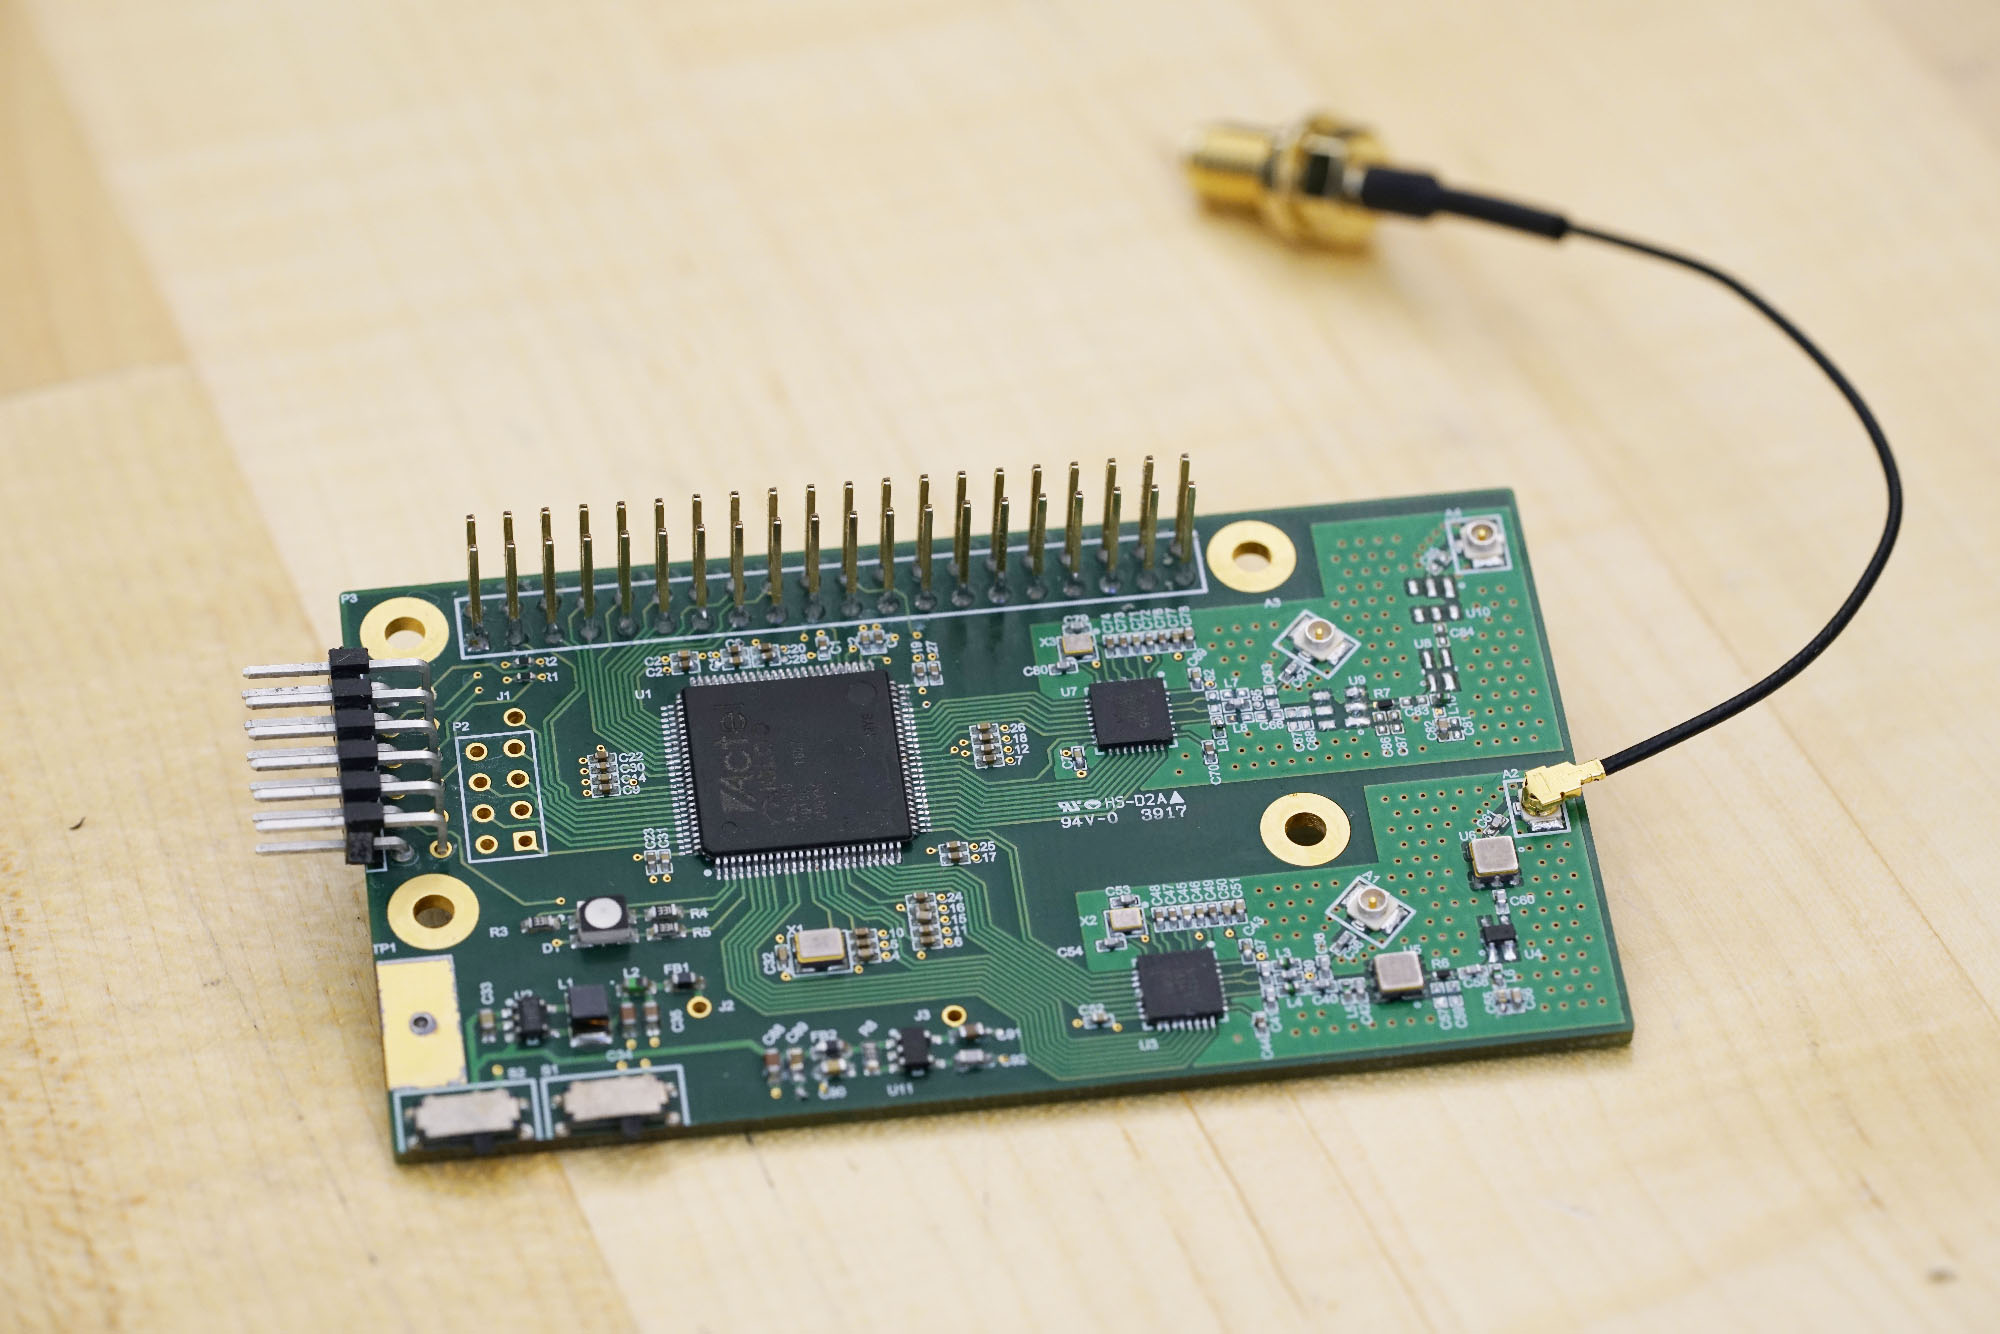
\includegraphics[width=0.5\linewidth]{figures/gw-anon-sm}
    \\
    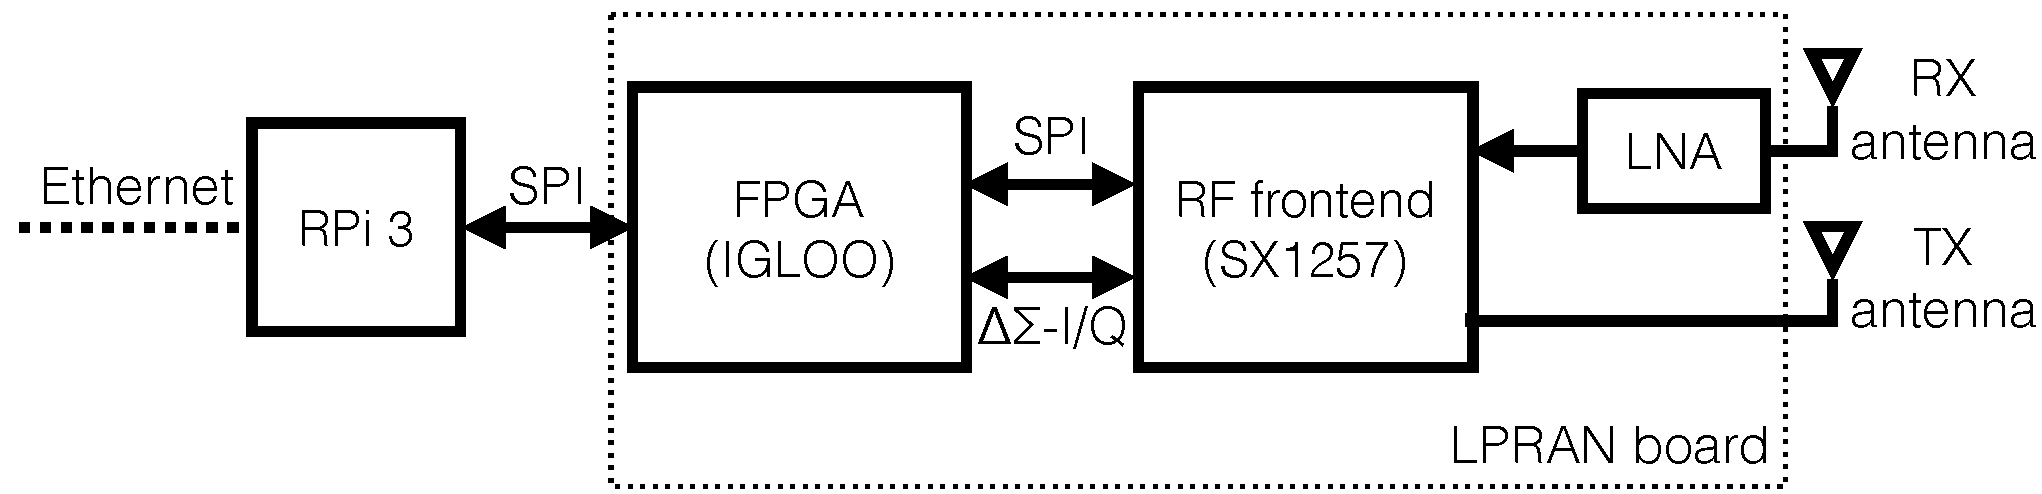
\includegraphics[width=0.8\linewidth]{figures/lpran-block_cropped}
    \caption{The LPRAN board and its functional block diagram.}
    \label{fig:lpran-photo}
\end{figure}

\begin{figure}[!htb]
    \centering
    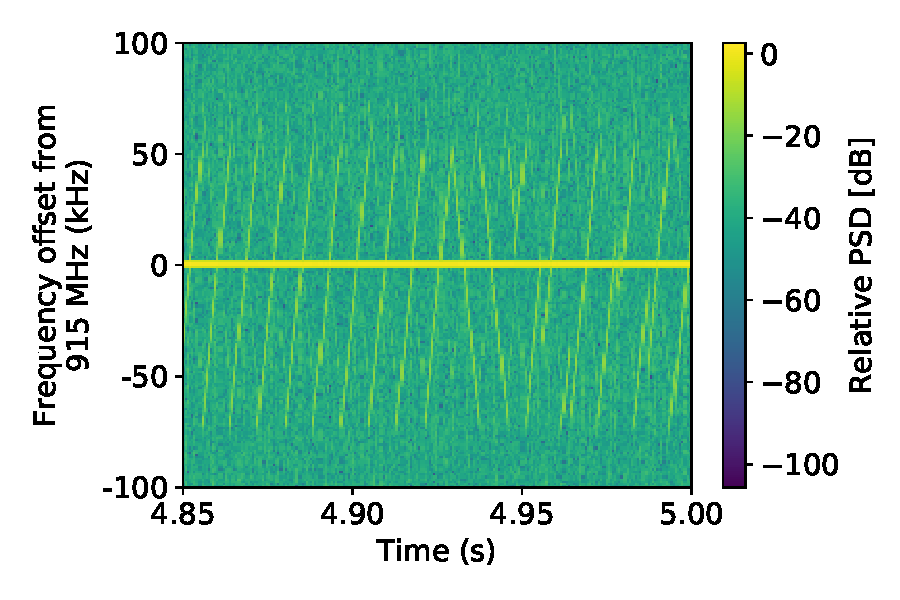
\includegraphics[width=0.8\linewidth]{figures/LPRAN_spectrogram}
    \caption{The spectrogram of a weak LoRa transmission captured by the LPRAN device.}
    \label{fig:lpran-spectrogram}
\end{figure}

\subsection{OpenChirp Architecture}
\label{sec:oc-arch}

\begin{figure*}[!htb]
    \centering
    \begin{minipage}[c]{.65\textwidth}
        \centering
        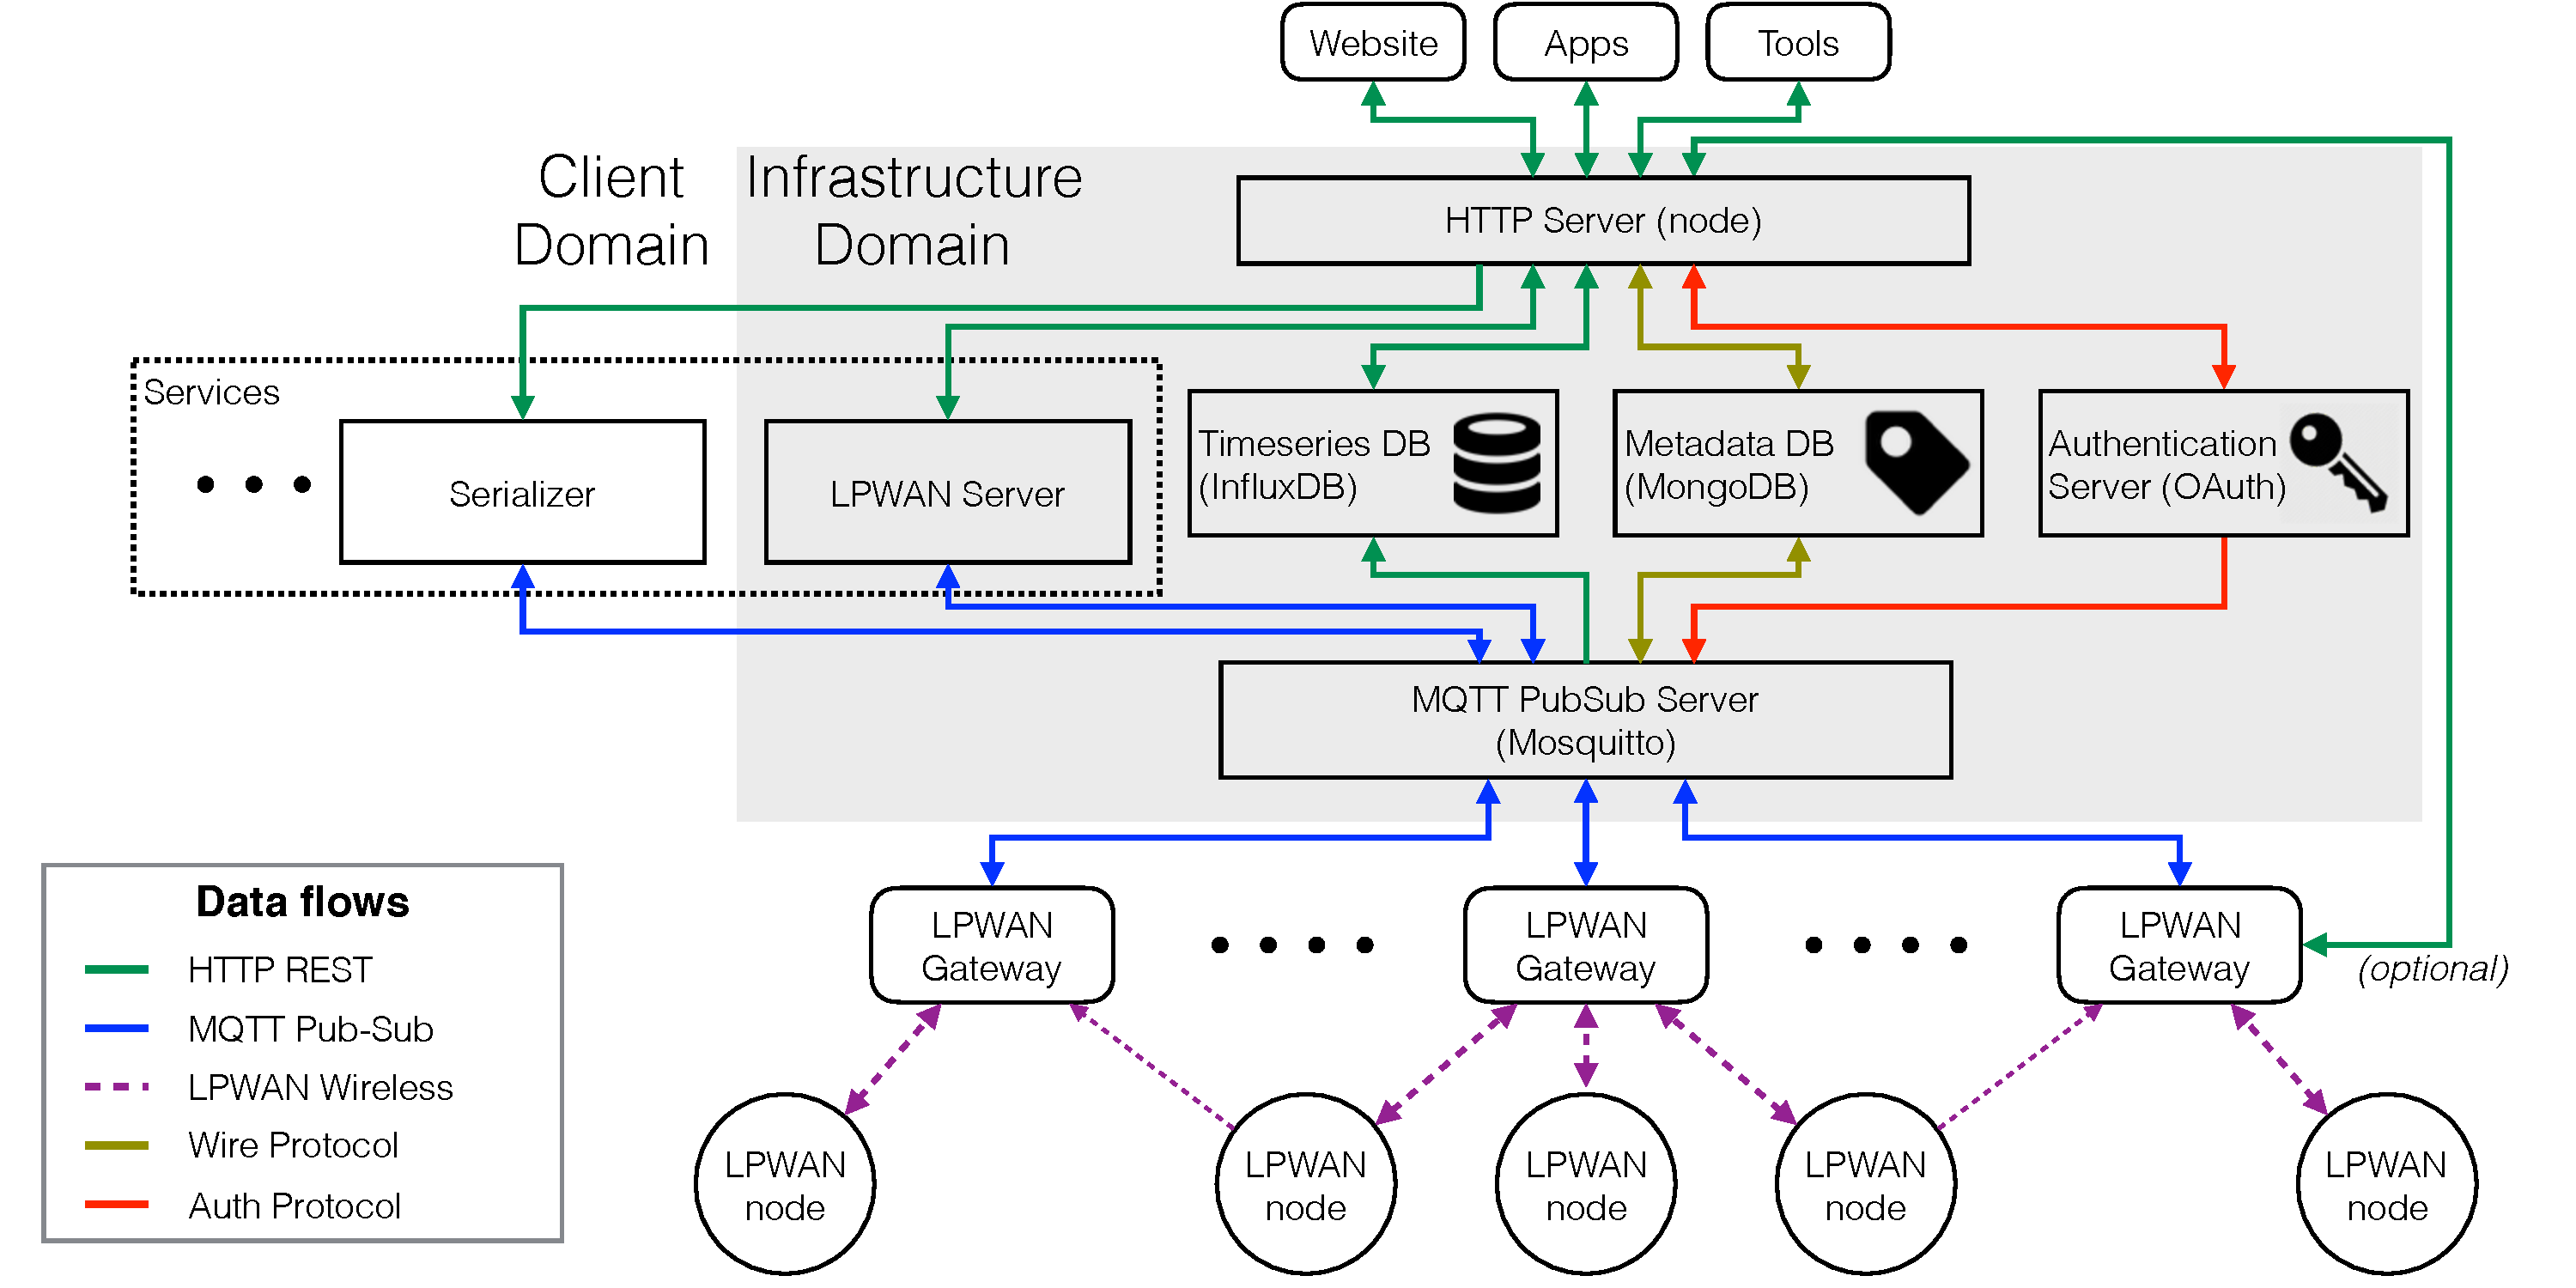
\includegraphics[width=\linewidth]{figures/openChirp_architecture}
        \caption{The OpenChirp Architecture}
        \label{fig:oc-arch}
    \end{minipage}%
    \begin{minipage}[c]{.35\textwidth}
        \centering
        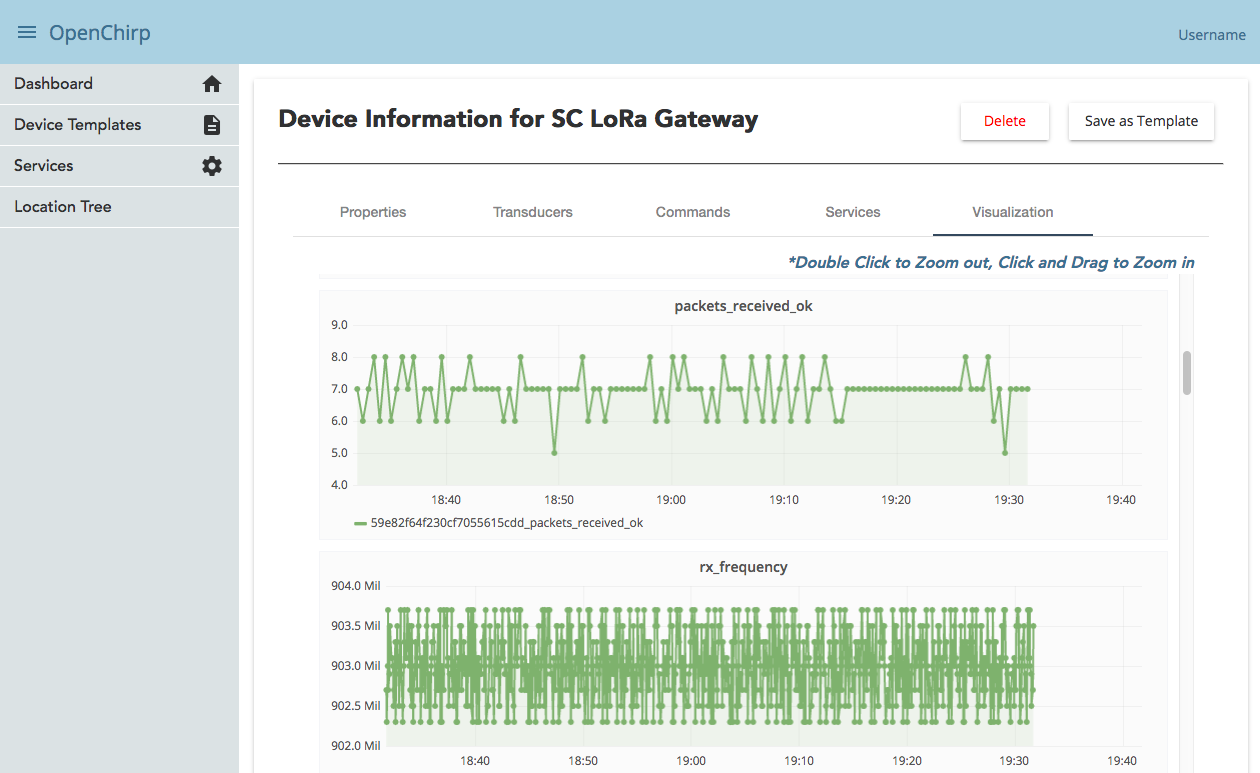
\includegraphics[width=\linewidth]{figures/OC_screenshot}
        \caption{Screenshot of OpenChirp's web interface showing a typical
        visualization of data from a LoRaWAN gateway}
        \label{fig:oc-screenshot}
    \end{minipage}
\end{figure*}

OpenChirp~\cite{dongare2017openchirp} is a completely open, end-to-end LPWAN
architecture with the goal of simplifying the design and deployment of
Internet-of-Things (IoT) devices. It currently supports the LoRa LPWAN
(LoRaWAN) protocol~\cite{LoRaWanAlliance2015}, with future plans to support
Bluetooth 5, IEEE 802.15.4 and other IoT communication protocols. OpenChirp
aims to be easily deployable as a private or public network, with complete
access to all frontend and backend components including the web interface,
various data management services and APIs. Existing LPWAN solutions currently
do not provide access to all components in their systems.

OpenChirp's modular and scaleable architecture is shown in \figref{oc-arch}.
An instance of OpenChirp can be accessed at \texttt{http://www.openchirp.io}.
Next we describe some of it's important components.


\subsubsection{MQTT interface}
All LoRaWAN wireless devices communicate with gateways, which forward their
data over the MQTT publish-subscribe protocol. MQTT communication is managed
by a Mosquitto MQTT broker. Though only one broker is currently supported,
further development is being made to support bridging multiple MQTT brokers
together. Each device is represented by a topic to which various services,
users and other devices could publish or subscribe to. LoRaWAN's Ack-based
re-transmission and MQTT's quality-of-service parameter ensure reliable
transport of data between wireless devices and the cloud. All IoT devices are
expected to communicate to OpenChirp through the MQTT interface.

\subsubsection{HTTP REST interface}

Users interact with OpenChirp through an HTTP REST interface. This
includes operations such as adding and configuring devices and
gateways, generating unique device IDs and access tokens, downloading data
published by a given device, etc. Various web interfaces, command line tools
and apps are expected to interact with OpenChirp through the REST interface.
All HTTP requests are handled by a node server.

\subsubsection{Services}

Services are responsible for acting on incoming data and performing various
operations on it. They enable adding intelligence to an otherwise simple
network. Devices register to available services when they are configured,
which informs a service to publish or subscribe to it's topics. Services can
then perform important operations, such as store data, generate plots, extract data packet etc. based on incoming data or user requests. A LoRAWAN server
service~\cite{loraserver} and data storage service (implemented with InfluxDB)
are already implemented and activated in OpenChirp. Other services such as a
deserializer to unpack data and a GPS mapping service can also be enabled.
Additionally, custom services can be developed using an open API and run on
any external servers.

\subsubsection{Authentication and Sharing}

Authentication is managed by OAuth integration to Google accounts. Further
developments are being made to allow other options like LDAP, etc. OpenChirp
allows sharing devices and device data between users. To share a device, the
device owner can provide publish and subscribe access to a device's topics.

\subsubsection{Web Interface}

The web interface provides a rapid way to login to OpenChirp, add and manage
devices and to visualize various forms of data gathered by devices. An example
of the web interface implemented with AngularJS is shown in
\figref{oc-screenshot}.

\subsection{LPRAN Architecture}
\label{sec:lpran-arch}

LPRAN, shown in \figref{lpran-photo}, is an auxiliary hardware module
developed for LPWAN gateways, which mimics the functionality of a
software-defined radio at a significantly lower-cost. By providing access to
raw radio signals, it enables interesting application like coherent
combining~\cite{charm2018underreview}.

LPRAN's high-performance radio frontend is a Semtech SX1257~\cite{sx1257} chip
(that can detect signals up to -30 dB below the noise floor) that outputs the raw radio I/Q
signals as a sigma-delta modulated stream. An on-board FPGA and Raspberry Pi 3
perform additional signal processing to convert the stream into a usable form.
An example of a signal captured by the LPRAN hardware is shown in
\figref{lpran-spectrogram}.

\section{Demonstration}
\label{sec:demo}

We demonstrate various software and hardware components to aid the rapid
deployment and management of a LoRa LPWA research network.

\subsection{OpenChirp Interface}
\label{sec:oc-interface-demo}

We will demonstrate the ease and simplicity of adding and managing LoRaWAN
devices as well as gateways using the OpenChirp network interface. We plan to
deploy multiple wireless LoRa devices (both commercial-off-the-shelf PyCom
LoPy and custom LoRaBug devices) across the demo area and be able to log and
visualize data using OpenChirp.


\subsection{LPRAN Micro-SDR Platform}
\label{sec:lpran-demo}

We will demonstrate a combination of a LPRAN board and a Raspberry Pi 3
listening to a LoRa transmission and providing the raw radio signals as well
as a spectrogram of the reception.

\section*{Acknowledgment}

The authors would like to thank everyone working on OpenChirp, Prof. Swarun Kumar
for various insights about the physical layer, Orne Brocar for developing the
LoRa server, and {\color{red} XYZ} agency.


\bibliographystyle{unsrt}
\bibliography{references} % references.bib is the name of the Bibliography in this case

\section{Demo Requirements}
\label{sec:requirements}

The demonstration requires a power connection (with multiple plugs), a screen,
keyboard and mouse. A stable internet connection would be preferable, but not
essential. This demonstration will use multiple battery-powered wireless
transmitters in the 868 MHz ISM spectrum.

\end{document}


